\clearpage
\section{细铁丝的阴影}
一张宽 1\,024 像素的贴图，每四列画一列铁丝，其余三列透明。让相机和点光源停在同一个位置，近看贴图中间的十二列。画面上可以数出三根铁丝，每根约三个屏幕像素宽。点击铁丝能选中网片，可是在改前的墙面图里，三根铁丝都没有影子。

\begin{figure}[H]\centering
\begin{tabular}{@{}ccc@{}}

\includegraphics[width=.28\linewidth]{../../../output/validation/fine-mask/before-raster.png}&

\includegraphics[width=.28\linewidth]{../../../output/validation/fine-mask/before-wall.png}&
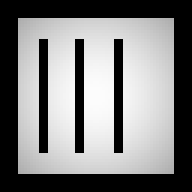
\includegraphics[width=.28\linewidth]{../../../output/validation/fine-mask/after-wall.png}\\
\small 相机看到的铁丝&\small 修复前的墙面&\small 修复后的墙面
\end{tabular}
\caption{三张图来自同一机位。第一张显示相机看到的实心部分，后两张只显示同一面白墙收到的直接光。观察中央的三条竖线。}
\end{figure}

沿着射线找到三角形，着色器会在交点处读取透明度。那次错误发生得更早，在 CPU 准备这张图时，程序把宽度缩到了 512。设小图的列号为 $j$，从 0 开始。旧代码取每一格的中心，到原图里只读一列，因此取到的原图列号是
\[
  \left\lfloor (j+\tfrac12)\frac{1024}{512}\right\rfloor = 2j+1.
\]
于是留下的是第 1、3、5、7 列，而铁丝恰好都在第 0、4、8 列。显卡拿到的小图里已经没有铁丝了。即使后来准确找到了交点，读到的透明度也一直是零。\href{run:../validation/fine-mask/before.json}{改前读数}

\begin{center}
\begin{tikzpicture}[x=.79cm,y=.58cm,font=\small]
\node[anchor=east] at (-.18,1.42) {原图列号};
\node[anchor=east] at (-.18,.42) {原图};
\node[anchor=east] at (-.18,-.68) {旧代码读取};
\foreach \i in {0,...,11}{
  \node at (\i+.5,1.42) {\i};
  \draw[draw=line,fill=pale] (\i,0) rectangle ++(1,.85);
}
\foreach \i in {0,4,8}{\fill[blue] (\i+.04,.04) rectangle ++(.92,.77);}
\foreach \i in {1,3,5,7,9,11}{\draw[-{Stealth[length=1.6mm]},muted] (\i+.5,-.9)--(\i+.5,-.03);}
\end{tikzpicture}
\end{center}
\note{蓝格是铁丝，浅格是透明处。箭头指向旧代码读过的列。项目按测试贴图重画。}

这张图既有颜色，也有透明度。墙面反射的颜色仍可以从小图取。判定射线有没有碰到铁丝时，需要保留原图的透明度。为此，模型加载器给缩小过的镂空贴图另存一个通道，每个原始像素用一个字节。底色图取透明通道 A，独立的透明贴图取红通道 R。同一张图整片透明或整片不透明时，缩小后读到的值处处相同，可以省下这份空间。

\clearpage
\subsection{从贴图到墙上的阴影}
显卡以 32 位整数读取材质数据，一个整数可以放四个透明度值。若要读另存的透明图的第 6 个字节（从 0 数起），整数下标就是 $6\div4$ 的商 1，取其中第 $6\bmod4=2$ 个字节。一个字节能表示 0 至 255，除以 255 后便得到材质使用的 0 至 1。把四个相邻位置分别读出，再按交点离它们的距离混合，就能沿用原来的透明度裁剪规则。\href{https://www.pbr-book.org/4ed/Textures_and_Materials/Image_Texture}{PBRT 第四版，第 10.4 节}

\begin{Code}
// AlphaMask.glsl / maskTexel，节选。image.x 是这张图的起点。
uint word = texels[image.x + byteIndex / 4u];
// 每个字节占 8 位，右移后用 255（最低八位全为 1）取出该字节。
return float((word >> (8u * (byteIndex % 4u))) & 255u) / 255.;
\end{Code}

在图中第 $(26,32)$ 个像素，相机看到的是 $z=1$ 处的铁丝。旧版的射线一直走到 $z=0$ 的墙，墙面的红通道读到 0.25468，和移走铁丝时一样。修复后，射线先碰到铁丝，墙上的直接光变为 0。底色图自带透明度、另配一张透明图、用 OBJ 的 \code{map\_d} 导入透明图，这三种材料各有 342 个先前出错的像素，现在逐个与相机看到的实心部分相符。\href{run:../validation/fine-mask/after-replay.json}{RenderDoc 事件和像素读数}

烘焙测试把灯牌放在网后方，读取网前同一枚探针的 64 条光线。在没有铁丝时，其中 20 条能到达灯牌。放回铁丝，只有 5 条到达。灯牌的红光强度为 4，因此探针记下的红通道从 $4\times20/64=1.25$ 变为 $4\times5/64=0.3125$。两张透明图只在原图的偶数列有差别，旧程序却允许它们共用一个烘焙文件。现在显卡读取的完整透明度也参与文件校验，放回原图能重新读回与它相符的烘焙。\href{run:../validation/fine-mask/after.json}{探针与烘焙文件}

\subsection{一个像素覆盖多根铁丝时}
把同一张纹理的 1\,024 列铺进约 38.63 个屏幕像素，每个像素横向覆盖约 26.51 列。相机此时读取预先缩小的纹理层（mipmap）。RenderDoc 中第 4、5 层的透明度都是 $64/255\approx0.251$，与铁丝占原图面积的四分之一很接近。但材质要求透明度至少达到 0.5，每个像素都会被略过。固定机位的 1\,444 个网片像素，光栅绘制和拾取都没有留下铁丝。阴影射线逐条查原图，仍在 342 个位置被挡住。这是另一个可以单独复现的远景问题。\href{run:../validation/fine-mask/far-after-replay.json}{远景截帧中的纹理层}\quad\href{run:../validation/fine-mask/far-after.json}{远景读数}

\begin{figure}[H]\centering
\begin{tabular}{@{}cc@{}}

\includegraphics[width=.21\linewidth]{../../../output/validation/fine-mask/far-after-raster.png}&
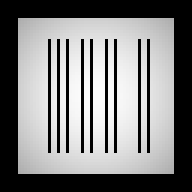
\includegraphics[width=.21\linewidth]{../../../output/validation/fine-mask/far-after-wall.png}\\
\small 相机未画出铁丝&\small 白墙上的阴影
\end{tabular}
\caption{相机和网片保持原位，只改变贴图在网片上铺开的范围，模拟远处的取样间距。左图用白色标记画出来的铁丝，因此整张图为黑色。右图每个像素只发一条阴影射线，粗条纹标出本次取样碰到铁丝的位置。}
\end{figure}

使用原来的单点绘制缓慢后退，从每个像素横跨 1.75 个纹素起，铁丝连续 91 帧消失。改为缓慢横移，铁丝在测试区域内应当占约四分之一，实际画面却在 12.5\% 与 25\% 之间跳了 16 次。现在打开“SSAA 2×2”，四处取样后分别给铁丝和墙着色，同一段后退中每帧都能看到铁丝。两层错开的网仍可能遮住同一处样点。\href{run:Redflag-Technical-Decisions-Updated.pdf}{方案与实拍}\quad\href{run:../validation/mask-footprint-compare-rank/report.json}{竖纹、横纹和斜纹的读数}
